\chapter{Suites et séries de fonctions}
\labch{suites_et_series_de_fonctions}

Le Calcul infinitésimal est l'apprentissage du maniement des \emph{inégalités} bien plus que des égalités, et on pourrait de résumer en trois mots:
\begin{center}
        MAJORER, MINORER, APPROCHER.
\end{center}

V.1 Écart de deux fonctions de \cite{calcul_infinitesimal} \\
De même qu'on cherche à \emph{approcher} un \emph{nombre} inconnu (défini par un procédé quelconque) à l'aide de nombres décimaux (ou rationnels), de même il est naturel en Analyse de chercher à \say{ approcher } une \emph{fonction} complexe inconnue (qui peut être définie par des procédés variés, somme de série, intégrale dépendant d'un paramètre, solution d'équation différentielle, etc.) à l'aide de fonctions que l'on considère comme \emph{connues} (polynômes, fonctions exponentielles, fonctions trigonométriques, etc.). Mais il faut préciser ce qu'on entend par \say{ approcher }, c'est-à-dire \say{ mesurer } en quelque sorte l'\say{ écart } de deux fonctions, de même que la valeur absolue $|x-y|$ mesure l'écart de deux nombres réels ou complexes. \\
L'idée la plus naturelle est que si une fonction $g$ \say{ approche } une fonction $f$ dans un ensemble $E$ où elles sont toutes deux définies, alors, pour chaque $x_0 \in E$, la \emph{valeur} $g(x_0)$ de $g$ doit \emph{approcher} la \emph{valeur} $f(x_0)$ de $f$ au sens usuel, c'est-à-dire que $|f(x_0)-g(x_0)|$ doit être \say{ petit }. Comme ceci doit avoir lieu en \emph{chaque} poit $x_0$ de $E$, on est conduit à prendre pour \say{ écart } de deux fonctions complexes $f$, $g$ définies dans $E$ le nombre
$$d(f, g) = \sup_{x \in E} |f(x)-g(x)|.$$
Lorsqu'il s'agit de fonctions \emph{réelles} $f, g$ définies dans un intervalle $E = [a, b]$ de $\R$, l'idée d'\say{ écart } que nous venons de définir peut se concrétiser graphiquement de la façon suivante: dire que $d(f,g) \leqslant \varepsilon$ signifie que pour tout $x \in E$ on a $g(x)-\varepsilon \leqslant f(x) \leqslant g(x) + \varepsilon$, c'est-à-dire que le graphe de $f$ est \emph{tout entier} contenu dans le \say{ bande } de demi-largeur $\varepsilon$ autour du graphe de $g$. \\
Pour distinguer cette idée d'\say{ approximations } d'autres notions que nous examinerons plus tard \textcolor{red}{à réécrire}, nous dirons qu'il s'agit d'\emph{approximation uniforme} d'une fonction par une autre dans un ensemble $E$ où elles sont toues deux définies; il est important de remarquer que cette notion \emph{dépend essentiellement} de l'ensemble $E$ que l'on considère: si $f$ et $g$ sont toutes deux définies dans un ensemble plus grand $E'$, la relation $|f(x) - g(x)| \leqslant \varepsilon$ pour $x \in E$ n'entraîne nullement $|f(x)-g(x)| \leqslant \varepsilon$ pour $x \in E'$. \\
Étant donnés deux ensembles de fonctions $\mathscr{F}$ (les fonctions \say{ inconnues }) et $\mathscr{G}$ (les fonctions \say{ connues }) toutes définies dans un même ensemble $E$, nous dirons pour abréger qu'\emph{on peut approcher uniformément dans} $E$ les fonctions de $\mathscr{F}$ par les fonctions de $\mathscr{G}$ si, pour toute fonction $f \in \mathscr{F}$ et \emph{tout nombre} $\varepsilon > 0$, il existe une fonction $g \in \mathscr{G}$ (dépendant de $f$ et de $\varepsilon$) telle que l'écart $d(f,g) \leqslant \varepsilon$, c'est-à-dire que 
$$|f(x) - g(x)| \leqslant \varepsilon \quad \text{pour tout } x \in E.$$


\begin{tikzpicture}
    \begin{axis}[width=6.5cm,
        axis lines=middle,
        grid=major,
        xmin=-0.1, xmax=1.1,
        ymin=-0.1, ymax=1.1,
        % xlabel=$x$, xlabel style={right},
        % ylabel=$y$, ylabel style={above},
        tick style={thick},
        ticklabel style={font=\normalsize},
        xtick={0, 1}, 
        ytick={0, 1},
        % legend entries={0.5x},
            legend style={
            at={(1.05,0.4)},
            anchor=north,
            legend columns=1},
            legend cell align={left}
    ]
    
    \def\a{-0.1}
    \def\b{1.1}
    \def\eps{0.5}
    
    \addplot[blue,thick,samples=100,domain=0:\b] {x^3+x-2} {};

    \end{axis}
\end{tikzpicture}

\newpage

\section{Théorème d'approximation de \textsc{Weierstrass}}
Aussi connu sous le nom  de \emph{théorème de \textsc{Stone-Weierstrass}}

\begin{theo}
    Toute fonction continue sur un segment $[a, b]$ de $\R$ à valeurs dans $\R$ ou $\C$ est limite uniforme sur $[a, b]$ d'une suite de polynômes.
\end{theo}

\begin{preuve}
    \cite{calcul_infinitesimal} page 157.
\end{preuve} 

L'exercice suivant montre qu'il existe une suite de polynômes $(P_n)$ qui converge uniformément vers la fonction racine carrée sur $[0, 1]$.

\begin{exercice}
    \emph{Exercice 5. TD Ch. VIII}\\
    Soit la suite de fonctions définie pour tout $x \in [0, 1]$ par
    $$
    \begin{cases}
        P_0(x) &= 0,\\
        P_{n+1}(x) &= P_n (x) + \frac{1}{2} \big( x-P_n (x)^2 \big).
    \end{cases}
    $$
    Montrer que $(P_n)$ converge uniformément vers une fonction $f$ sur $[0, 1]$.
\end{exercice}

\begin{marginfigure}[-5cm]
	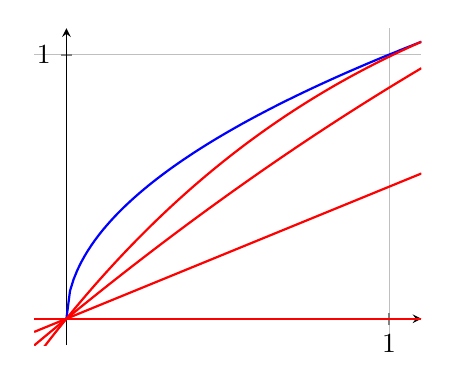
\begin{tikzpicture}
    \begin{axis}[width=6.5cm,
        axis lines=middle,
        grid=major,
        xmin=-0.1, xmax=1.1,
        ymin=-0.1, ymax=1.1,
        % xlabel=$x$, xlabel style={right},
        % ylabel=$y$, ylabel style={above},
        tick style={thick},
        ticklabel style={font=\normalsize},
        xtick={0, 1}, 
        ytick={0, 1},
        % legend entries={0.5x},
            legend style={
            at={(1.05,0.4)},
            anchor=north,
            legend columns=1},
            legend cell align={left}
    ]
    
    \def\a{-0.1}
    \def\b{1.1}
    
    \addplot[blue,thick,samples=100,domain=0:\b] {x^(1/2)};
    \addplot[red,thick,samples=100,domain=\a:\b] {0};
    \addplot[red,thick,samples=100,domain=\a:\b] {x/2};
    \addplot[red,thick,samples=100,domain=\a:\b] {-1/8*x^2+x};
    \addplot[red,thick,samples=100,domain=\a:\b] {-1/128*x^4+1/8*x^3-5/8*x^2+3/2*x};
    \end{axis}
\end{tikzpicture}


%import matplotlib.pyplot as plt
%import numpy as np
%from numpy.polynomial import Polynomial

%PAS = 1e-3
%n = 8
%X = np.arange(0, 1, PAS)


%P = Polynomial([0])
%plt.plot(X, P(X))

%for k in range(n):
%    P = P + 1/2 * (Polynomial([0, 1]) - P ** 2)
%    plt.plot(X, P(X))

%racine = [np.sqrt(x) for x in X]
%plt.plot(X, racine, 'r')
%plt.show()

\end{marginfigure}

Peut-on génraliser à $\R$ ? \dots

\begin{prop}
    Si $(P_n)_{n \in \N}$ est une suite de polynômes convergeant uniformément sur $\R$ vers une fonction $f$, alors $f$ est un polynôme.
\end{prop}

\begin{preuve}
    Source : \cite{exos_oraux} \& \cite{maths-france}. \\
    Soit $(P_n)_{n \in \N}$ une suite de polynômes convergeant uniformément sur $\R$ vers une fonction $f$. \\
    D'après la critère de \textsc{Cauchy} uniforme, il existe un rang $n$ tel que pour tout $p \in \N$, 
    $$\Ninf{P_{n+p} - P_n} \leqslant 1.$$
    La fonction polynomiale $P_{n+p} - P_n$ est donc bornée sur $\R$ autrement dit elle est constante. On a alors,
    $$\forall (p, x) \in \N \times \R,\ P_{n+p}(x) = P_n(x) + P_{n+p}(0) - P_n(0) \xrightarrow[p \to + \infty]{} P_n(x) + f(0) - P_n(0)$$
    donc par unicité de la limite simple, $f : x \mapsto P_n(x) + f(0) - P_n(0)$, qui définit bien une fonction polynomiale. 
\end{preuve}

\section{Approximation polynomiale de \textsc{Bernstein}}
\emph{Exercice 10. TD VIII} \\
\underline{Démonstration:} \cite{calcul_infinitesimal} page 159.

\begin{tcolorbox}
    Soit $f$ une fonction $k$-lipschitzienne sur $[0, 1]$. Le polynôme de \textsc{Bernstein} d'ordre $n$ associé à $f$ est le polynôme
    $$\Bernstein_n(f)(x) = \sum_{k=0}^{n} f \left( \frac{k}{n} \right) \binom{n}{k} x^k (1-x)^{n-k}$$
    La suite $(\Bernstein_n(f))_n$ des polynômes de \textsc{Bernstein} converge uniformément vers $f$ sur $[0, 1]$. \\
    \textit{Ce résultat s'étend à toute fonction continue sur un segment à valeurs dans $\C$}.
\end{tcolorbox}

Le sujet X/ENS PSI 2018 propose une élégante démonstration de ce résultat d'analyse pure en passant par les probabilités. (Je crois que la version du TD est un peu différente).
    
\begin{box_enonce}
    
    Préciser les hypothèses sur $f$.
        
    Soit $x \in ]0, 1[$ et $n \in \Ne$. On considère $X_1, \dots, X_n$ des variables aléatoires mutuellement indépendantes et suivant toutes la même loi de \textsc{Bernoulli} de paramètre $x$. On pose
    $$S_n = \frac{X_1 + \cdots + X_n}{n}.$$
    \begin{enumerate}
        \item Exprimer $\E(S_n)$, $\V(S_n)$ et $\E(f(S_n))$ en fonction de $x$, $n$ et du polynôme $\Bernstein_n(f)$.
        \item En déduire les inégalités:
        $$\sum_{k=0}^{n} \left| x- \frac{k}{n} \right| \binom{n}{k} x^k (1-x)^{n-k} \leqslant \V(S_n)^{1/2} \leqslant \frac{1}{2\sqrt{n}}.$$
        \item Montrer que $\lambda^\alpha \leqslant 1+\lambda$ pour tout réel $\lambda > 0$ et en déduire l'inégalité:
        $$\left|x-\frac{k}{n} \right|^\alpha \leqslant n^{-\alpha/2} \Bigg(1 + \sqrt{n} \left|x - \frac{k}{n} \right| \Bigg)$$
        pour tout $x \in ]0, 1[, n \in \Ne$ et $k \in \llbracket 1, n \rrbracket$.
        \item Soit $n \in \Ne$. Montrer que 
        $$\Ninf{f-\Bernstein_n(f)} \leqslant \frac{3k}{2} \frac{1}{n^{\alpha/2}}.$$
        Conclure.
    \end{enumerate}
\end{box_enonce}

\section{Intégration d'une série de fonctions}
Soit $S:x \to \sum\limits_{n=1}^{+\infty} \frac{(-1)^n}{1+n^2 x^2}$.
\begin{itemize}
    \item Donner l'ensemble de définition de $S$ et donner un équivalent en $+\infty$.\\
    $\blacktriangleright$  $D_S = \Re$.\\
    $\blacktriangleright$ On se doute que $S$ \textbf{se comporte comme} $\frac{1}{x^2}$ en $+\infty$. L'idée est donc de déterminer la limite de $x^2 S(x)$ en $+\infty$. Le \textbf{théorème d'interversion des limites} permet d'affirmer que cette limite est finie et qu'elle est égale à $c = \sum\limits_{n=1}^{+\infty} \frac{(-1)^n}{n^2}$. Une séparation des termes pairs et impairs de la somme (et le résultat du \href{https://fr.wikipedia.org/wiki/Problème_de_Bâle}{problème de Bâle}) permet de montrer que $c = -\frac{\pi^2}{12}$ et donc $S(x) \sim_{+\infty} -\frac{\pi^2}{12x^2}$.
    \item Montrer que $S$ est intégrable sur $\Rpe$ et calculer $\int_0^{+\infty} S(t) \mathrm{d}t$.\\
    $\blacktriangleright$ Comme $S$ est une série alternée, on peut lui appliquer le \textbf{théorème des séries alternées} et écrire que 
    $$|S(x)| \leqslant \frac{1}{1+x^2} \text{ (majoration du reste d'ordre 1)}$$
    L'intégrabilité du majorant sur $\Rpe$ assure celle de $S$ sur cet ensemble. \textcolor{green}{Est-ce que l'intégrabilité sur R+* des termes de la somme et leur CU vers $S$ impliquent l'ingrabilité de $S$ sur cet ensemble ? c.f. théorème de la convergence dominée peut-être...}\\
    $\blacktriangleright$ L'interversion série/intégrale permet de montrer que $\int_0^{+\infty} S(t) \d t = \frac{\pi}{2} \sum\limits_{n=1}^{+\infty} \frac{(-1)^n}{n} = -\frac{\pi}{2} \ln(2)$ (c.f. \nameref{deux_sommes}).\\
    \textcolor{green}{Dans la correction (p. 374), on effectue le calcul sur une somme partielle et on détermine ensuite la limite de cette somme. J'avais naïvement travailler avec l'intégrale jusqu'en +infini et la somme aussi, \textbf{est-ce licite ?}}.
\end{itemize}

\section{Équivalent d'une série de fonctions}
\begin{exercice}
    On pose $f(x) = \sum\limits_{n=1}^{+\infty}\frac{x}{n(1+nx^2)}$. Donner un équivalent de $f$ et $0^+$.
\end{exercice}

\begin{solution}
    Éffectuer une comparaison série/intégrale aux termes de la somme pour encadrer $f$ (ne pas oublier de justifier l'intégrabilité des fonctions sur $[1, +\infty[$):
    $$\int_{2}^{+\infty} \frac{x}{t(1+tx^2)} \d t + \frac{x}{1+x^2} \leqslant f(x) \leqslant \int_{1}^{+\infty} \frac{x}{t(1+tx^2)} \d t + \frac{x}{1+x^2}.$$ 
    Décomposer les intégrandes en éléments simples et calculer les intégrales:
    $$-2x \ln(x) + o_0(x\ln(x)) \leqslant f(x) \leqslant -2x \ln(x) + o_0(x\ln(x))$$
    Finalement, 
    $$f(x) \isEquivTo{0^+} -2x\ln(x)$$
\end{solution}

\section{Série de fonctions continues dont la somme est discontinue}
\begin{prop}
    \marginnote[0cm]{\cite{contre-exemples} p.257}
    Soit la suite $(f_n)_{n \geqslant 0}$ d'applications continues de $[0,1]$ dans $\R$, de terme général
    \begin{alignat*}{2}
        f_n\ :\ [0,1]\ &\longrightarrow\ \R\\
        x\ &\longmapsto\ f_n(x) = (1-x)x^n.
    \end{alignat*}
    La somme des $f_n$ est discontinue.
\end{prop}

\begin{preuve}
    Pour tout point $x$ de $[0,1[$, la série $\sum f_n(x)$ est le produit par $(1-x)$ d'une série géométrique de raison $x$ où $0 \leqslant x < 1$, donc elle converge et sa somme est égale à $(1-x)/(1-x) = 1$. De plus $f_n(1) = 0$ pour tout entier naturel $n$. La série de fonctions $\sum f_n$ converge donc simplement sur le segment $[0,1]$ et sa somme est l'application 
    \begin{alignat*}{2}
        S\ :\ [0,1]\ &\longrightarrow\ \R\\
        x\ &\longmapsto\ S(x) =
        \begin{cases}
            1 &\text{ si } x \in [0,1[,\\
            0 &\text{ si} x = 1,
        \end{cases}
    \end{alignat*}
    qui est discontinue en $1$.
\end{preuve}


\section{Convergence uniforme d'une suite de fonctions polynomiales}
Soient $(P_n)_n$ une suite de fonctions polynomiales de $\R$ dans $\R$.\\
On suppose que $(P_n)_n$ converge uniformément vers une fonction $f$ sur $\R$. Montrer que $f$ est une fonction polynomiale. 
\begin{itemize}
    \item $(P_n)_n$ CU donc il existe $n \in \N$ tel que pour tout $p \in \N$, $\Vert P_{n+p}-P_n \Vert_{\infty} \leqslant 1$. 
    \item ...
\end{itemize}

\section{Fonction \texorpdfstring{$\zeta$}{zêta} alternée}
\marginnote[0cm]{\emph{Exercice 13. TD VIII}}
On définit la fonction $\zeta$ alternée $F$ comme suit
$$\boxed{F(x) = \sum_{n=1}^{+ \infty} \frac{(-1)^{n-1}}{n^x}}.$$
\begin{itemize}
    \item Déterminer l'ensemble de défintion de $F$ et trouver une relation entre $F$ et $\zeta$.
    \begin{itemize}
        \item Calculer $\zeta(x) - F(x)$ pour trouver que $\zeta(x) = \frac{1}{1-2^{1-x}} F(x)$.
    \end{itemize}
    \item Déterminer $\displaystyle \lim_{x \to 1} (x-1) \zeta(x)$.
    \begin{itemize}
        \item En comparant $\zeta$ à une intégrale, on peut montrer que $\frac{1}{1-x} \leqslant \zeta(x) \leqslant \frac{1}{1-x} + 1$.
    \end{itemize}
    \item On peut aussi procéder de la manière suivante: $\zeta$ est décroissante sur $]1, +\infty[$ donc $\zeta$ admet une limite $\ell \in \Rp \cup \{ + \infty \}$ en $1$.\\
        $\blacktriangleright$ Si $\ell \in \Rp$, par passage à la limite dans l'inégalité $\zeta(x) \geqslant \sum\limits_{n=1}^{N} \frac{1}{n^x}$, $$\ell \geqslant \sum\limits_{n=1}^{N} \frac{1}{n} \xrightarrow[N \to + \infty]{} +\infty.$$ 
        Donc $\ell = + \infty$ et $\displaystyle \lim_{x \to 1} \zeta(x) = +\infty$. 
    \item Déterminer $\displaystyle \lim_{x \to +\infty} F(x)$ ainsi qu'un équivalent de $\zeta$ en $+\infty$.
    \begin{itemize}
        \item On peut montrer que (\textcolor{green}{à détailler}) $\zeta(x) \sim_{+ \infty} 1$.
    \end{itemize}
\end{itemize}

\section{Fonctions continues nulle part dérivables}
\epigraph{\emph{``Je me détourne avec effroi et horreur de cette plaie lamentable des fonctions continues qui n'ont point de dérivées.''}}{--- Charles \textsc{Hermite} (1893)}
    
\epigraph{\emph{``C’est un cas où il est vraiment naturel de penser à ces fonctions continues sans dérivées que les mathématiciens ont imaginées, et que l’on regardait à tort comme de simples curiosités mathématiques, puisque l’expérience peut les suggérer.''}}{--- Jean \textsc{Perrin} \footnote{Physicien, chimiste et homme politique français (1870 - 1942), prix Nobel de physique 1926.}, au sujet du mouvement brownien}
    
- thème Ch. 8 \\
- DS MPSI 2015 \\
- \url{https://share.miple.co/content/XEZ7y9BayeSN1} \\
- \url{http://christophebertault.fr/documents/articles/Article - Une famille nombreuse de fonctions continues partout derivables nulle part.pdf}

\begin{itemize}
    \item Intégrale à paramètre vs. série de fonctions
    \item Développements asymptotiques de sommes de séries de fonctions
\end{itemize}

%\begin{figure}[!h]
%   \begin{floatrow}
%\ffigbox{\input{bolzano-lebesgue}}%
%        {\caption{first figure}\label{fig:example-1}}
%\hfill
%\ffigbox{\input{blanc-manger}}%
%        {\caption{second figure}\label{fig:example-2}}
%   \end{floatrow}
%\end{figure}

Pour découvrir d'autres \emph{courbes remarquables}, lire le paragraphe éponyme dans \cite{contre-exemples} page 350. 
